\chapter{LUX-ZEPLIN Simulations}
\label{chap:lz_simulations}
\par
In this chapter, important contributions to the development of the LZ simulation capabilities are described.
All the contributions are specifically for BACCARAT (described in the previous chapter).
These include updates to a light map for S2 photons and early development work to migrate a subset of simulations onto graphics card processors.
Finally, updates to a background particle generator are discussed, which is used in subsequent chapters.
Sections of this work were supported by Oracle Cloud Computing and have been presented by the author in \cite{se_poster_2018,se_poster_2019_summerschool,se_poster_2019_bristol,SEriksen_IoP_2021_talk_ref}.

\section{S2 Light Map}
\label{sec:s2lightmap}
\par
A single free electron simulated in the LXe with accelerate upwards towards the gas layer due to the electric field.
Once in the gas, the mean photon yield per electron is 825 \cite{NoPhotonsPerElectron}.
As a single scatter event can produce in excess of dozens of electrons, the number of photons which need to be simulated quickly becomes unmanageable, creating a simulation bottleneck.
\par
To get around this, a probabilistic map is used to determine the photon hit pattern on the PMTs and flight time.
For the S2 signal, this is broken up into two sets of probability density functions (PDF).
The first is the likelihood of a photon hitting a given PMT from a given position.
This is essentially the number of photons which hit this PMT divided by the number of photons which hit any PMT.
The second is the likely path taken by the photon, as this effects the time it takes for the photon to hit the PMT, and thus the resultant waveform.
\par
In order to create this light map, large scale simulations of the photons have to be performed at least once.
For every simulation after the map has been generated, there is a significant speed increase as the photons themselves no longer need to be simulated.
In the subsequent simulations, the electron paths are stopped once they reach the liquid surface.
The position of the electron is used to determine the path it would have taken and points along this path are taken to be the photon origin. % to the anode.
The maps are then used along with random numbers and binary searches to determine which PMT the photon hit (if any) as well as how long it took.

\par
A notable downside of this approach is that for different scenarios one may wish to investigate (such as using a different purity of Xenon or the temperature and therefore pressure) then a new light map is needed to account for these effects.
A version of this approach had been used within BACCARAT for a number of years \cite{lz_simulations_ref}, but was outdated due to detector design changes.
The S2 Light Map now in use within BACCARAT, created by the author, took into account the latest geometry and detector physics.

\subsection{S2 Radial Variation} \label{sec:s2radialvariation}
\par
The electric field originates from three electrodes: a cathode grid just above the bottom PMTs, a gate grid just below the surface of the liquid Xenon, and an anode grid in the gaseous Xenon.
In previous simulations it was assumed that the anode and gate were both rigid structures and so had a fixed distance, and electric field between them.
In this case, the number of photons produced in the gas gap by an electron is given by \autoref{eq:s2lightmap_nophotons} and is equal no matter the distance from the centre:
\begin{equation}
    N_{photons/e} = eep \times (\alpha \times E_{gas} \times 1000 - \beta \times P - \gamma) \times d_{gas}
    \label{eq:s2lightmap_nophotons}
\end{equation}
Where $\alpha$, $\beta$ and $\gamma$ are constants, $E_{gas}$ is the electric field in the gas, P is the pressure of the liquid, and $d_{gas}$ is the distance from the top of the liquid to the anode \cite{NoPhotonsPerElectron}.
$eep$ is the electron emission probability at the surface.
%is taken from PiXeY data and fitted to give $eta = -0.03754 \times (eliq^{2}) + 0.5266 \times eliq - 0.84645$, where $eliq$ is the electric field in the liquid Xenon \cite{ElectronExtractionEfficiency}.
The emission probability is included as we want to use the average number of photons per electron.
This simplification was known to be incorrect as a stronger signal\footnote{more photons being detected} should be observed in the detector centre.
Tests conducted at SLAC indicated that there is bending of the wires according to \autoref{WireDeflection} due to the electric field.
\begin{equation}
    x(r,E) = A \sqrt{ \bigg( 1 + \cos{ \Big( \frac{r \pi}{R} } \Big) \bigg) \bigg( B^2 + r^2 \bigg) } \bigg( e^{(r-C)} + 1 \bigg)^{-1} 
    \label{WireDeflection}
\end{equation}
Where R is the radius of the wire, r is the point on the wire and A, B and C are all of the form: $A(E) = \sum_{j=0}^{M} a_{j} E^{j}$. E is the electric field and $a_{j}$ are constants.
As such, the electric field is not constant with radius and thus the number of photons produced by electroluminescence is changed.
\par
These changes were implemented into the simulation package as a scaling on the number of photons which the S2 Light Map is probed for.
Implementing it in this way allows for the resultant signal size to scale with the electric field without having to require a dynamically changing detector grid geometry - which is a much more complex approach.


\section{Graphics Card Simulations}

\par
The probabilistic approach described in the previous section created a significant performance increase. 
However, there are several significant factors which limit the feasibility of using similar methods for the rest of the detector, including;
\begin{itemize}
    \item Optical propagation is required to be performed at least once
    \item Other regions of the detector contain significantly more complex geometry
\end{itemize}
For example, if a probabilistic map were to be applied to the entire TPC Liquid Xenon region, several weeks worth of a full cluster would be required in order to produce the equivalent statistics.
Although there are ways in which this could be reduced - such as Z-line symmetry - the initial overhead remains impractically high.

\subsection{Geant4 Simulations}
\par
Before attempting to improve the speed of simulation, it is important to understand why simulation speed is limited. 
LZ particle propagation simulations are performed in BACCARAT, a software package built upon GEANT4.
In GEANT4, a detector is defined by solid-based modelling or CSG (Constructed Solid Geometry) \cite{geant4_geometry_ref}.
A detector (or scene) is defined by a set of primitive volumes that can be described by some parameters.
An example of this is a sphere; a primitive solid that can be described by a single parameter; radius.
Primitives can be rotated, displaced and combined with other primitives via boolean operations to create more complex solids such as that shown in Figure \ref{fig:csg_geometry_example}.
\begin{figure}[!htbp]
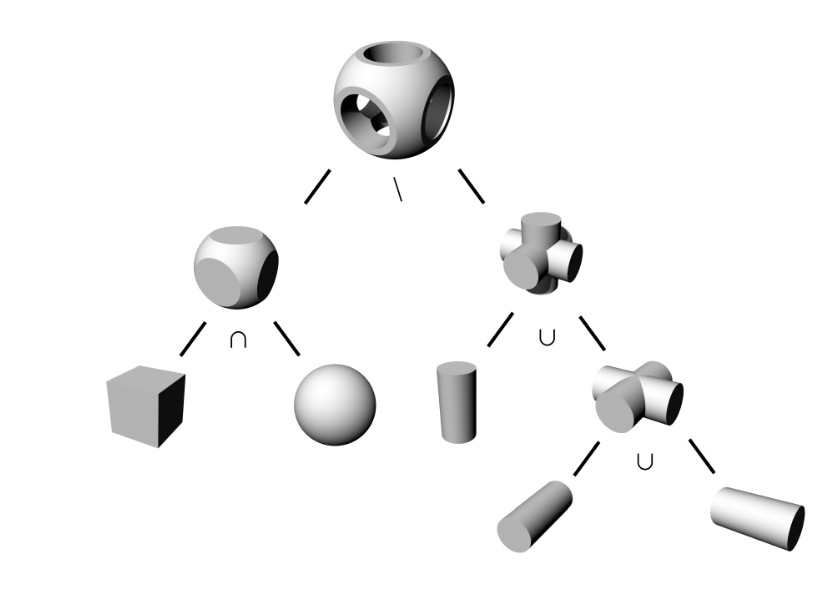
\includegraphics[height=8cm]{Figures/Simulations/csg_geometry.png}
\centering
\caption{Complex solid created from 5 primitive solids using boolean operations; union $\cup$, intersection $\cap$ and difference \textbackslash. Adapted from \cite{csg_geomtry_ref}}
\label{fig:csg_geometry_example}
\end{figure}

\par
In application, the primitive is defined by more than the basic shape parameters (such as radius).
The parameters are used in combination with functions so properties of the solid can be attained.
For example, the solid must be implemented in such as way that it is possible to determine if a point $\vec{x}$ is within the solid, and whether a ray travelling in direction $\hat{d}$ will intersect with the surface of the solid.
These functions have to account for all relevant calculations that relate to a solid.
\par
All of the solids in a scene are contained within a geometry tree.
The top of the tree contains the 'world' volume, inside which there are daughter volumes (which do not overlap with each other).
These volumes can contain there own daughters, and so on.
To the user, this structure is often less obvious with solids connected to each other by logical volumes (LV) and physical volumes (PV).
LVs contain information associated with a solid such as material. 
PVs can contain one or more LV which are given positions are rotations inside of it. 
A PV can be part of a higher up LV.
\par
When a particle is simulated, its track starts inside a volume of a solid which is in the geometry tree.
In the direction of travel, a check must be performed to determine intersections with the volume as well as all immediate daughter volumes.
As each daughter is a subtraction in volume of it's parent, the number of interactions is generally limited.
Even so the number of sibling volumes is often a reliable indicator of particle tracking performance.
Therefore it is logical to for the tree to be as narrow as possible to reduce the number of sibling volumes.
This can be at odds with how a detector is designed, such as if a solid has to have holes for other solids to pass through.
The problem with this is that interior of the solid isn't fully defined by the volume anymore\footnote{An example of this in LZ geometry are the calibration tubes, passing through the water tank, outer detector, and OCV}.
In this case, the geometry tree is widened so that volumes inside become siblings of the problem volume, which in turn increases the number of intersection calculations.
This must be the case to enforce the requirement that each volume is contained entirely by it's mother volume and that it does not overlap with siblings.
\par
GEANT4 in part mitigates this by separating the geometry tree nodes into perpendicular facing boxes, called voxels \cite{geant4_voxel_ref} which are not part of the detector volumes.
During particle propagation, the voxels are checked first for intersections.
If there is an intersection, the detector volumes contained within that voxel are then checked.
Though useful, the voxels are limited to a single level, is performed iterative (1 axis at a time) to save memory and so can hit computation speed.
The GEANT4 approach can be summarised as;
\begin{quote}
    A detector is a tree of nested solids, each composed of some material and mathematically implemented by a particular C++ class.
\end{quote}

\subsection{Optical Simulations}
\par
In addition to particle tracking, the GEANT4 must also handle particle interactions inside a volume which can result in daughter particles that also need to be tracked.
However, in LZ the bottleneck is in the photon propagation, taking up in excess of 95\% of computing time (after using the S2 Light Map).
Optical photon simulations are relatively simple in that no daughter particles that need to be tracked.
There is some probability of a photon being absorbed and re-emitted during propagation, but otherwise photon propagation can be simplified to travelling in a straight line until they reach a boundary.
The simulation is therefore dominated by intersection calculations, or \textit{"has the photon reached the edge of this volume yet?"}.
Therefore increasing the number of these intersection calculations per second will decrease the overall simulation time.
\par
GEANT4-based simulations are performed on CPUs which have typically been designed to minimise task latency; ie the time required to complete any given task.
Although it is possible to multi-thread simulations, it is rarely done due to simulation frameworks often originating decades ago.
An alternative processor widely available is a GPU, which is designed to maximum throughput.
This is achieved by having individual poorer thread performance but by having more threads available\footnote{Additionally, each task should be as independent as possible and require very few resources}.
If a simulation can be moved onto a GPU it will allow for more concurrent tasks that will massively outweigh the slower performance of each task, resulting in more simulations per second
\par
There have been many different attempts to transfer parts or entire simulations on to GPUs, such as Chroma \cite{chroma_whitepaper_ref}, ANTS2 \cite{ants2_whitepaper_ref}, Exascale Computing Project \cite{ExaSMR_whitepaper_ref} and MPEXS \cite{mpexs_whitepaper_ref}.
The majority of these make use of NVIDIA CUDA \cite{cuda_ref}, an application programming interface (API) allowing for GPU hardware to be used for general purpose computing.
\par
Chroma is of particular interest as it was proposed and designed for optical simulations, as it has been utilised in several experiments \cite{chroma_with_tpcs1_ref,chroma_with_tpcs2_ref,chroma_with_tpcs3_ref}, and has more recently received attention by gen-3 direct detection dark matter \cite{DARWIN_GPU_simulations_2022_ref}.
Chroma uses surface-based modelling where a triangle mesh describes the geometry.
This tessellation reduces the number of primitives to one, a triangle which is defined within a the users program in CUDA.
As the surface of a solid is described by a finite set of triangles, this naturally leads to curves not being represented as accurately as the GEANT4 method.
To some extent this can be mitigated by increasing the density of the of primitives, but this is a trade off between accuracy and performance.
The complete geometry is typically defined as a union of non-intersecting closed meshes.
\par
As the geometry structure is broken during tessellation there is no geometry tree which can be navigated.
As a result, Chroma implements a bounding volume hierarchy (BVH) tree structure, a method well used in industry \cite{real_time_collision_detection_ref}.
Crucially, as it is well tested there efficient ways of navigating it.
In a BVH, the lead nodes contain subsets of primitive lists.
To determine if there is an intersection in a BVH, starting at the root node a test is done for an intersection with the box associated with that node.
If an intersection is found, the children are tested for an intersection - analogous to the GEANT4 voxel approach.
The number of intersection calculations is dependant upon the depth of the tree and the number of children per node.
An example BVH is shown in Figure \ref{fig:bvh_example}.
\par
When a simulation wants to be performed, the photon is first generated on the CPU and then copied over to the GPU for propagation.
When the photon is stopped generally by being absorbed at a surface, it is transferred back to the CPU.
Chroma has been shown to be 50-200x speed improvement when compared to GEANT4 single-core processing \cite{chroma_whitepaper_ref,chroma_presentation_ref}.
\begin{figure}[!htbp]
    \centering
    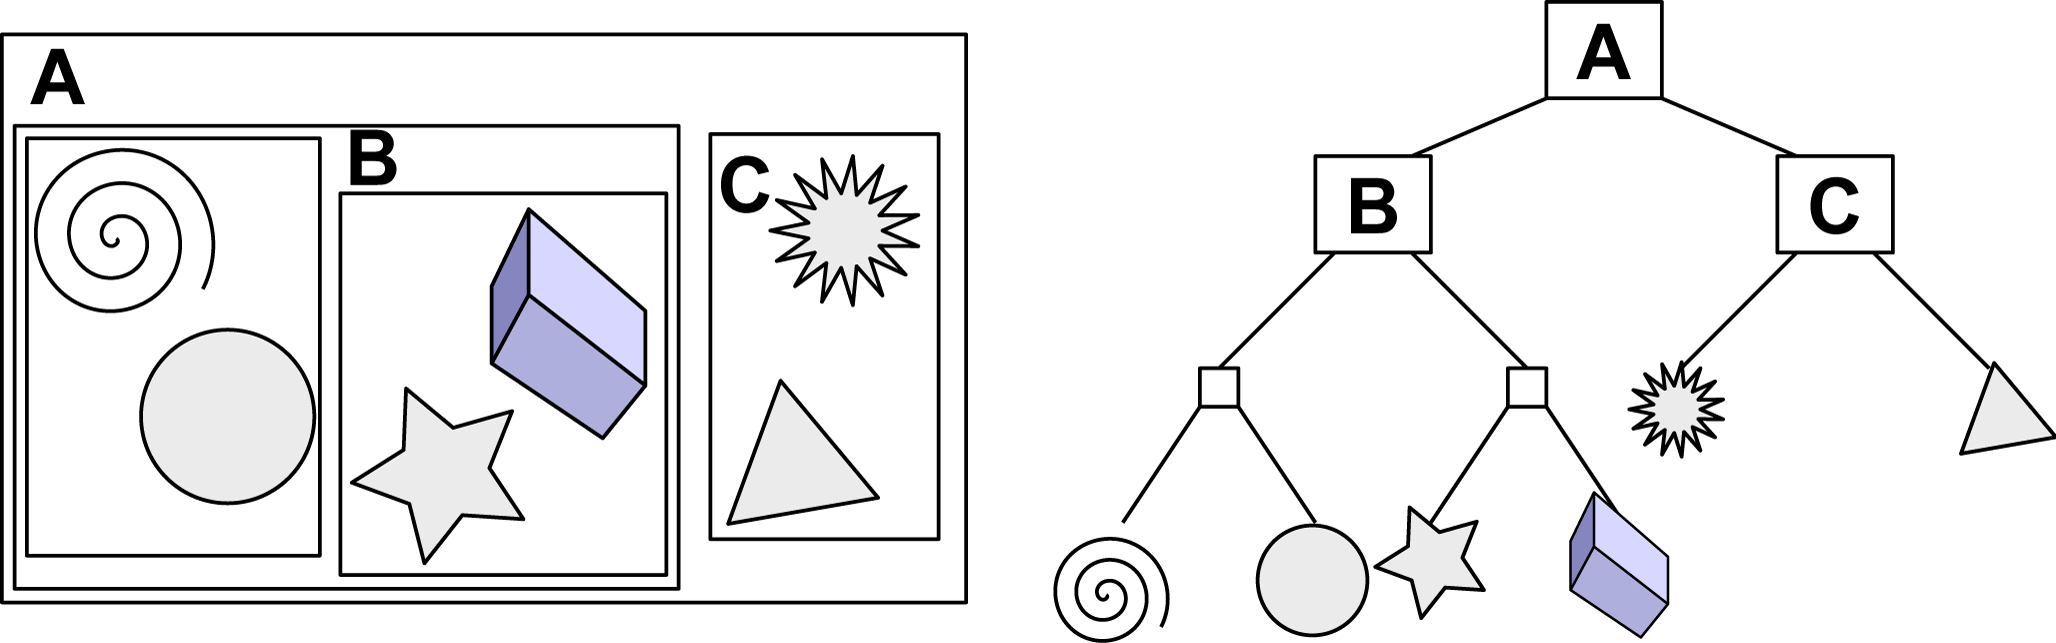
\includegraphics[width=\textwidth]{Figures/Simulations/bounding_volume_hierarchy.png}
    \caption{Example of 2D bounding volume hierarchy. 
             \textbf{Left:} the spacial relationship between solids and bounding volumes.
             \textbf{Right:} the intermediate nodes and the solids in the tree.
             From \cite{bounding_box_ref}}
    \label{fig:bvh_example}
\end{figure}
\par
Despite this, Chroma has some significant drawbacks.
Firstly, the code-base is in python, which makes integration within GEANT4 simulation frameworks impractical which are C++.
Secondly, the inefficient handling of photon generation.
Copying information between the GPU and CPU should be minimised in order to increase performance.
Finally, although tessellation is adequate for some surfaces, many detectors are comprised of exclusively curved surfaces.
In order to achieve adequate accuracy, the number of primitives required begins to eliminate any gain in the processing.
Inspired by Chroma, a separate project was created called Opticks which aimed to tackle the limitations \cite{Opticks_Paper_2017_ref,Opticks_CHEP_2019_ref,Opticks_CHEP_2021_ref} which is what was chosen here.

\subsection{Opticks}
\par
Where as Chroma is built around CUDA, Opticks\footnote{Yes it is a confusing name} is built around NVIDIA OptiX \cite{nvidia_optix_paper_ref}, a ray tracing API.
As most ray-tracing algorithms require only a small set of operations, OptiX allows the user to build applications from a small set of CUDA programs.
These programs can define the ray generation, intersections with surfaces, camera characteristics and so on.
This means that a primitive can be defined mathematically correct.
Additionally, more complex solids can be created by CSG as in GEANT4.
The primitives are described as boundaries  \cite{real_time_collision_detection_ref}.
\par
OptiX uses an acceleration structure which sorts primitives into spatial groups.
This is then used by a traversal algorithm to search for primitives that potentially intersect with a ray\footnote{OptiX provides acceleration to the geometrical intersection, not the intersection itself.}.
All details of the creation and traversing of the acceleration structures are handled internally by OptiX using user defined bounding box programs.
The creation of these groups remain a key research area in ray tracing \cite{NVIDIA_OptiX_GPU_Ray_Tracing_ACM_paper_ref,accelerated_bvh_ref}.
\par
Opticks is an open-source framework designed to convert GEANT4 geometry into an appropriate GPU form and perform photon simulations.
This includes the detector geometry and optical properties.
To allow for this, Opticks has ported the majority of GEANT4 primitives into CUDA equivalent ones \cite{Opticks_CHEP_2019_ref}.
Opticks converts the geometry tree used by GEANT4 into a boundary based geometry model.
Each CUDA primitive is defined by an intersection calculation which are based of those in \cite{real_time_collision_detection_ref} and a bounding box program.
All possible intersection directions are defined for each primitive; ray inside travelling outward, ray outside travelling inward.
The intersection decision of a solid is based upon \cite{CSG_Intersection_ref}, using a recursive algorithm.
However, OptiX does not allow for recursive intersection programs, so Opticks uses a always-left traversal method creating an iterative approach.
\par
The resultant Opticks geometry tree is a set of binary trees with primitive leaves and operator nodes.
Practically speaking this is as a NumPy serialised arrays, where each solid is defined by it's own binary tree \cite{Opticks_Paper_2017_ref}, and these trees are indexed together based upon the structure.
The nodes contain an rotations.
Opticks navigates the binary tree via bitwise manipulation\footnote{parent $=i >> 1$, left child $= i << 1$, right child $(i<<1)+1$}.
This means that the tree height should be kept relatively low in order to reduce the number of bits required to navigate it.
As such, Opticks has a limit of 7 as $(1 << (7 + 1)) - 1 = 255$ which allows for comparison with 256-bit CPU approaches as well not limiting memory use.
Opticks achieves this on trees which are not already of this height by attempting to balance them.
This is described in more detail in the following section.
\par
During the geometry conversion, Opticks attempts to highlight duplicate solids.
This way, when the geometry is uploaded to the GPU, the tree only needs to be uploaded once, and instancing is used which provides some memory saving \cite{Opticks_CHEP_2019_ref}.
Opticks also allows for geometry caching via NumPy serialisation \cite{Opticks_Paper_2017_ref} to avoid having to perform this conversion which is often computationally intensive, more than once.
\par
In addition to the solids conversion, material and boundary properties are also translated as NPY which are indexed to which solids they refer to.
Separate CUDA programs handle the ray behaviour when influenced by these properties.
\par
A key benefit of Chroma over opticks is that it relies upon CUDA only, and is therefore not a significant challenge to port to OpenCL \cite{chroma_whitepaper_ref}.
This will allow for non-NVIDIA GPU workflows.
However, for the foreseeable future, the performance will still lack significantly behind OptiX.
Additionally, all of the clusters which LZ current use or plan to use contain NVIDIA GPUs, with the primary upcoming computing resource Perlmutter using NVIDIA A100 GPUs \cite{perlmutter_ref}.
\par
In the next sections the translation of the LZ geometry is described along with initial performance metrics.
The proposed integration into the LZ simulation framework is discussed in \cite{SEriksen_Opticks_CHEP_2021_ref}.

\subsection{LZ Geometry Conversion}
\par
In order to use the LZ geometry, it must first be extracted from GEANT4 where it is defined.
The simplest way to export a GEANT4 defined geometry is via a GDML (Geometry Description Markup Language) file \cite{GDML_USER_GUIDE_ref}.
GDML is a subset of XML which is designed to describe the geometry by describing a detector as a series of trees which correspond to the hierarchy of volumes \cite{GDML_USER_GUIDE_ref}.
A small exert of the LZ geometry GDML is shown below;
\begin{lstlisting}[backgroundcolor=\color{lightgrey},
                   language=XML, xleftmargin = 0.5cm]
<volume name="expHall_log0x1051db0">
  <materialref ref="vacuum0xea27f0"/>
  <solidref ref="expHall_box0x1152c20"/>
  <physvol name="subVol0x106c220">
    <volumeref ref="subVol_log0x1058260"/>
    <position name="subVol0x106c220_pos" unit="mm" x="0" y="0"
       z="1189.395000001"/>
  </physvol>
</volume>
\end{lstlisting}
In this extract, we can see the logical volume \textit{expHall\_log0x1051db0} which is filled with the solid box, \textit{expHall\_box0x1152c20}, that is made of a vacuum.
Inside this box a physical volume has been placed, \textit{subVol0x106c220} which contains the logical volume \textit{subVol\_log0x1058260}.
\par
The structure of the GEANT4 geometry is as PV/LZ/PV/LV which means that if put into a geometry tree that isn't in the same style as GEANT4 will require twice as many nodes to properly navigate it than is actually necessary.
As the PV contains the placement of the LV and what the sibling volumes are the PV placement information can be propagated into the LV and removed.

\par
The LZ detector contains a number of solids which are of significant complexity that the tree describing them is greater than 7 in depth.
These are typically unbalanced due to the way in which they were created in GEANT4, for example where a shape contains many holes (and therefore multiple subtractions).
These would likely have been implemented as one subtraction at a time from the primary solid.
A balanced approach would be to union subtractions together and then perform a single subtraction.
Figure \ref{fig:UnionSolidBinaryTree} describes a solid made up of 4 primitive solids an unbalanced and balanced tree.
During the geometry conversion, Opticks recognises large trees and attempts to balance them via De Morgan's law.
This results in a tree with only union, intersection operators and complemented primitives.
These complemented primitives are conceptually "inside-out", but are implemented as just flipping the solid normal and classifying an intersection "Miss" becoming a volume "Exit".
\begin{figure}[!htpb]
\centering 
\begin{tikzpicture}[level distance=1.5cm,
  level 1/.style={sibling distance=3cm},
  level 2/.style={sibling distance=1.5cm}]
  \node {u}
    child {node {u}
      child {node {u}
        child {node {ps}}
        child {node {ps}}}
      child {node {ps}}}
    child {node {ps}};
\end{tikzpicture}
\begin{tikzpicture}[level distance=1.5cm,
  level 1/.style={sibling distance=3cm},
  level 2/.style={sibling distance=1.5cm}]
  \node {u}
    child {node {u}
      child {node {ps}}
      child {node {ps}}
    }
    child {node {u}
    child {node {ps}}
      child {node {ps}}
    };
\end{tikzpicture}
\caption{Binary tree representation of a simple solid comprised of the union (u) of 4 primitive solids (ps). \textbf{Left:} Unbalanced tree. \textbf{Right:} Balanced tree.}
\label{fig:UnionSolidBinaryTree}
\end{figure}
\par
This approach works for most unbalanced trees, however it does work for some of LZs components.
Around the PMTs in the TPC exists a titanium plate and PTFE lining.
The titanium plate holds the PMTs in place, and the PTFE creates a reflective surface for photons on top of the titanium.
As the solids must have space for each PMT they are implemented as one solid with each hole subtracted out.
The tree for this (as defined in GEANT4) is shown in Figure \ref{fig:Opticks_unbalanced_shape}.
\begin{figure}[!htbp]
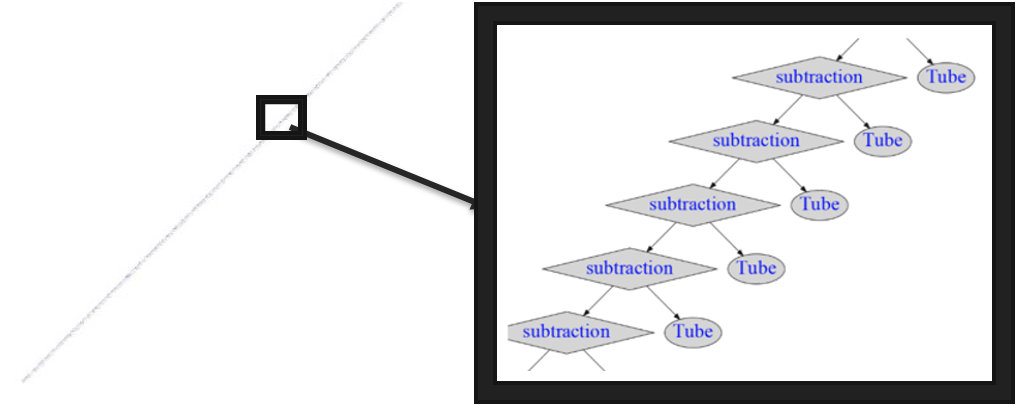
\includegraphics[width=\textwidth]{Figures/Simulations/unbalanced_ptfe.png}
\centering
\caption{Visual Representation of titanium top plate solid, comprised of a single G4Tube and 283 G4Tube subtractions. Kindly created by B. Krikler.}
\label{fig:Opticks_unbalanced_shape}
\end{figure}
For the top titanium plate this implementation would require $(1 << (253 + 1))-1 = 2^{254} - 1$ nodes, an impractically large number.
If perfectly balanced, this would still have a depth of 8.
This raises a problem as it requires the memory required to increases beyond a practical level with 512-bits required to describe the tree.
A method inspired by JUNO was adopted in order to handle this \cite{Opticks_CHEP_2021_ref}.
A primitive was created which defined the solids themselves, so rather than being comprised of a CSG tree of mulitple primitives, the trees became a single node of one primitive.
The basic creation process is shown in Figure \ref{fig:Opticks_PTFE_primative}.
In order the simplify the primitive code, the 3D shapes were reduced to 2D-intersections.
3D is then introduced by duplicating adding a Z-range in which the intersection needs to be evaluated.
Additional details of this approach at at \cite{optix_primitive_code_ref}.
Given the depth of these primitives, they were also likely a hold up in GEANT4 simulations, particularly the S2 light simulations mentioned in Section \ref{s2lightmap}.
In a branch of LZ code using GEANT4.10.6, these 4 solids were converted into G4MultiUnion solids which have built-in optimisation \cite{multiunion_ref}\footnote{At time of writing, LZ code uses GEANT4.10.3.p02 and this feature was introduced in GEANT4.10.4}.
This provided a 56\% decrease in simulation time.
\begin{figure}[!htbp]
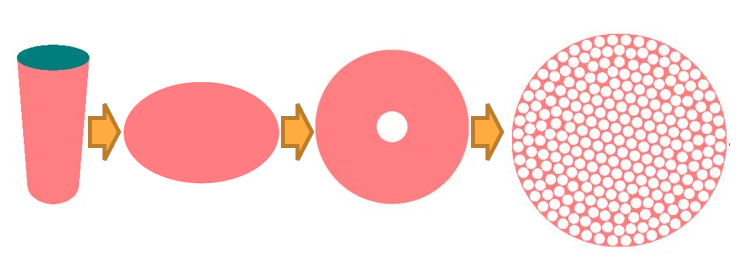
\includegraphics[width=0.7\textwidth]{Figures/Simulations/opticks_PTFE_primative.png}
\centering
\caption{Development stages for representing a 3D disc with multiple holes and a 2D disc with holes as defined within OptiX intersection program.}
\label{fig:Opticks_PTFE_primative}
\end{figure}

\par
The LZ geometry is comprised of in-excess of 900,000 shapes, and although there is some duplication, this only reduces down to around 14,000 shapes.
Given the complications with solids such as the titanium plate, then scope of the conversion was limited to just the TPC and Skin.
This to 9,000 unique shapes which is 30-times greater than that of experiments which have previous used Opticks such as JUNO and DayaBay \cite{Opticks_CHEP_2021_ref}.
The completed TPC conversion is shown in Figure \ref{fig:OpticksLZTPC}.
\begin{figure}[!htbp]
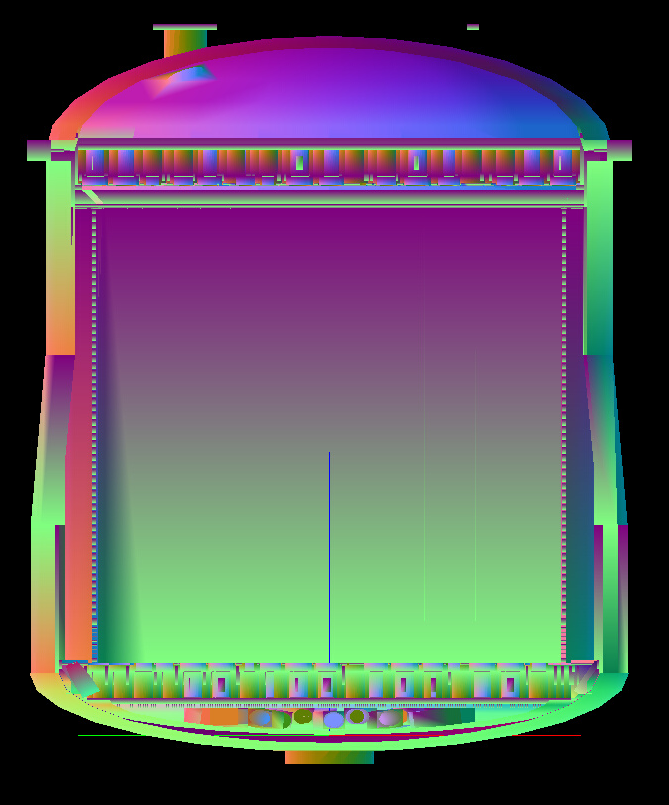
\includegraphics[width=8cm]{Figures/Simulations/LZ_In_Opticks.png}
\centering
\caption{TPC of LZ raytraced. Translated from Geant4 GDML file into NPY set using Opticks and viewed within Opticks via the OpenGL Buffer.
The blue, green and red lines towards the bottom of the figure are the axis.}
\label{fig:OpticksLZTPC}
\end{figure}

\subsection{Performance and Outlook}
\par
As LZ utilised multiple clusters across the globe, the computing environment is kept constant by use of containers.
As such, as part of this work Opticks was containerised \cite{opticks_docker_ref} which also acted in part as a way of removing legacy code and requirements.
NVIDIA OptiX 6.5.0 and CUDA 10.2 were chosen as they were the newest fully supported versions within the Opticks framework.
Making use of NVIDIA container runtime to access the GPU, the container was successfully run - with graphics - on a range of computing resources.
This allowed for integration into the LZ framework to begin, the plan for which is described in \cite{SEriksen_Opticks_CHEP_2021_ref,lz_status_with_opticks_ref}.
\par
As the geometry was cut down during the conversion, the most valuable test that could be performed was a comparison to the S2 Light Map (Section \ref{s2lightmap}).
For this, 200,000 photons per generated as a photon bomb as shown in Figure \ref{fig:OpticksLZTPC_S1_Photons}.
On a Tesla T4 GPU, after a 4-minute initialisation time using the serialised geometry, 200,000 photons per second were generated and propagated.
This marks a 720x improvement over single-core Geant4 propagation where 277 photons per second were generated and propagated for the S2 Light Map or 360x improvement over the expected gain when compared to GEANT4.
On the production clusters - such as Perlmutter - the performance is expected to increase.
This improvement highlights one of the reasons for choosing an OptiX-based approach rather than pure CUDA, as the improvement would have been closer to 200x such as was shown in \cite{chroma_presentation_ref}.
However, it still lacks behind the improvement demonstrated using Opticks in \cite{Opticks_CHEP_2019_ref}, though this is primarily due to higher grade GPUs being used with RTX-cores.
With the newer NVIDIA OptiX 7.0.0+, the algorithms are expected to continue to increase in speed which should provide additional performance.
Unfortunately the accuracy of this simulation has not been ascertained yet but the speed improvement is a promising result.
\begin{figure}[!htbp]
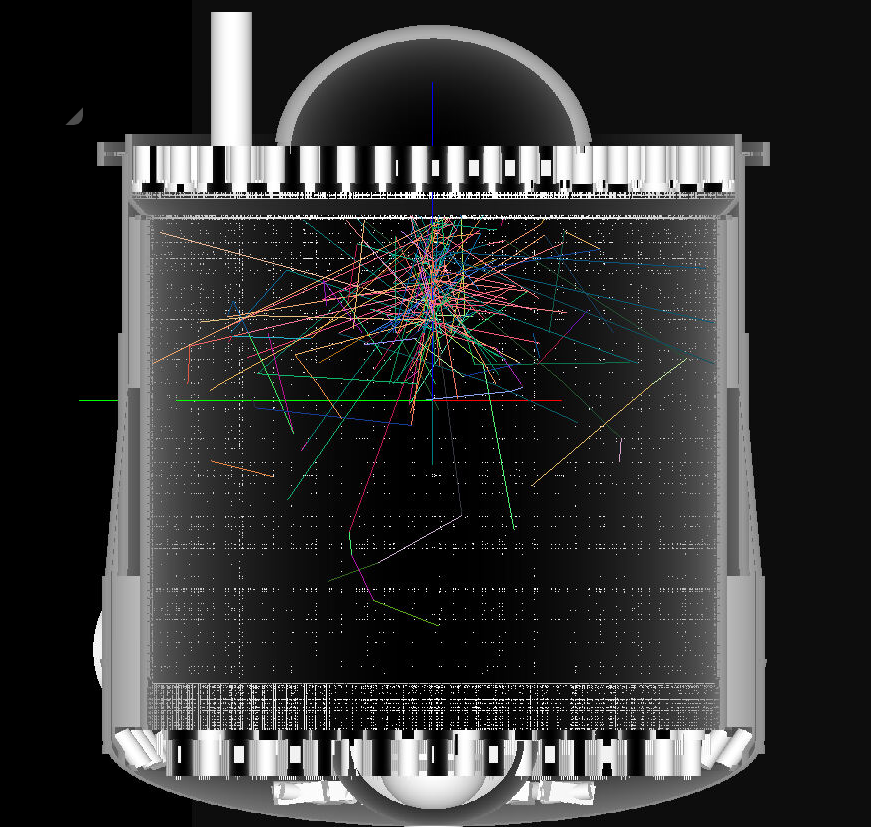
\includegraphics[width=10cm]{Figures/Simulations/LZ_S1_photons_In_Opticks.png}
\centering
\caption{TPC of LZ raytraced. Translated from Geant4 GDML file into NPY set using Opticks and viewed within Opticks via the OpenGL Buffer.
The blue, green and red lines extended outside the OCV are the axis. After each reflection a photons colour has been set to change.}
\label{fig:OpticksLZTPC_S1_Photons}
\end{figure}

\section{Cavern $\gamma$ Generator}
\label{sec:cavern_gamma_generator}

\par
Although the LZ detector has been constructed underground to limit cosmic radiation, it does come with a drawback of being in a mine with a non-negligibly radioactive rock and the shotcreat and gravel within the David Cavern.
LZ is not unique in this, it is a problem highlighted in a number of other underground experiments \cite{cavern_gamma_annual_modulation_CoGeNT_ref, cavern_gammas_in_Soudan_mine_ref}, with an annual modulation mimicking dark matter potentially seen in \cite{cavern_gamma_annual_modulation_CoGeNT_ref}.
The rate of this has been measured and can be attributed to the shotcreat and gravel \cite{LZ_Gamma_Ray_Background_ref}. 
One of the most significant sources of background come not from any internal component but rather from $^{238}U$, $^{232}Th$ and $^{40}K$ decays from the cavern in which the LZ detector exists \cite{LZ_Gamma_Ray_Background_ref}.
However, this is a computationally intensive process to simulation $\gamma$'s where the majority will not reach the actual detector.
To compensate, a generator for these $\gamma$'s was created - and originally described in \cite{rg_generator_ref} but summarised below.
The generator is a created by performing simulations of the decay chains originating in the shotcreat and gravel.
The $\gamma$'s which reach a pre-defined surface are saved.
A second stage simulation is then performed where each of the saved $\gamma$'s is generated a number of times and then saved at another pre-defined surface.
This boost occurs a number of times, until a generator surface.
When subsequent simulations are performed, these saved $\gamma$'s are randomly sampled. 

\par
In order to perform the For the creation of the generator additional cavern properties are added to the simulation.
Namely; a steel pyramid and gravel beneath the water tank, and a layer of shotcreat.
These adaptions are shown in Figure \ref{fig:Cavern_Geometry}.

\begin{figure}[!htbp]
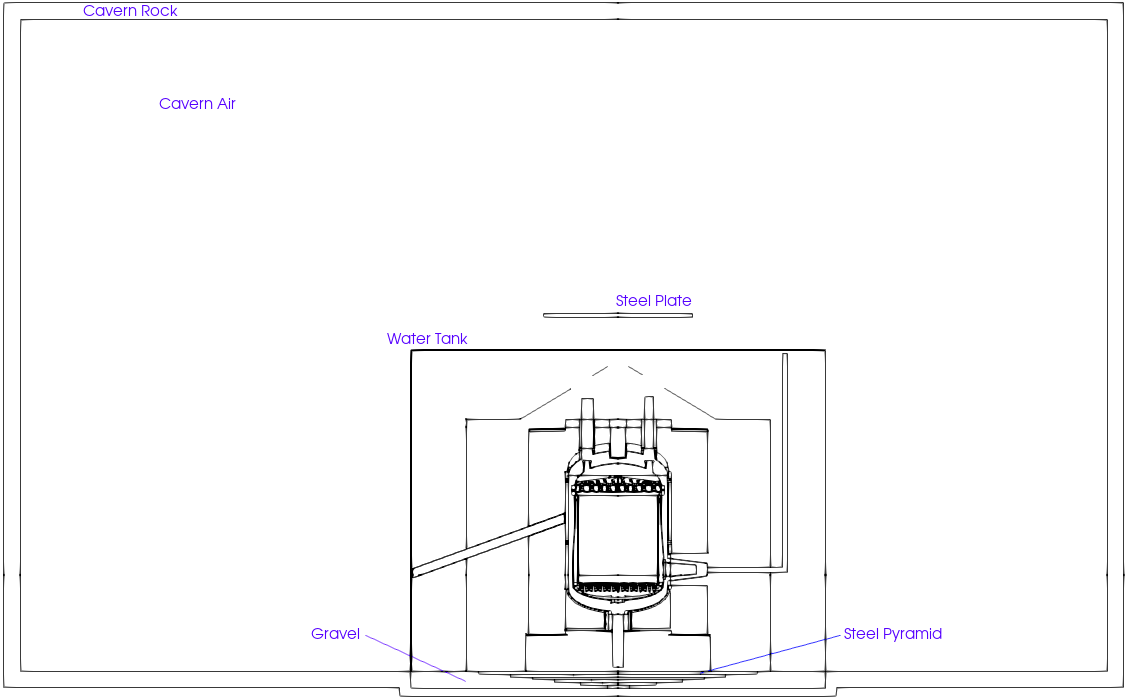
\includegraphics[width=\textwidth]{Figures/Geometry/cavern_geometry_with_markings.png}
\centering
\caption{LZ detector geometry slice with additional cavern geometry. OD PMTs are not seen present as they do not lie in this plane. The red dot marks (0,0,0).}
\label{fig:Cavern_Geometry}
\end{figure}

\par
Although as mentioned in \cite{scotthaselschwardt_thesis_ref}, a generator for the Davis Cavern $\gamma$'s existed, it had a number of flaws.
Firstly, no $\gamma$ below 2MeV was saved.
This meant that $^{40}K$ was not included and so the resultant expected rates being lower than expected.
Additionally, the generator was created using a version of GEANT4 which the rest of the simulation chain had moved on from; GEANT4.9.5 to GEANT4.10.3.p02. 
This motivated the creation of a new generator.

\par
The parameters of the new generator are shown in Table \ref{tab:cavern_gamma_generator_parameters} and a comparison of the energy distribution of the old and new generators is shown in Figure \ref{fig:cavern_gamma_energy_distribution}.
Although it can be seen that the previous generators had a maximum $\gamma$ energy of 10MeV, it also highlights a significant change between GEANT4.9.5 and GEANT4.10.3.p02.
That is, an increased rate above 9MeV.
These $\gamma$'s are predominately from ($\alpha$,$\gamma$) reactions such as $O + \alpha \to Ne + \gamma$.
These are of particular concern as they have the potential to mimic dark matter.
Conversely, they may produce large signals in the OD which would trigger a veto, reducing the detector livetime.
Since this version of GEANT4, there have been new studies of the ($\alpha$,$\gamma$) cross-section in other underground laboratories, such as in \cite{cavern_gammas_in_Soudan_mine_ref}.
Generally, very little attention has been given to ($\alpha$,$\gamma$) rates, and so it is possible that the observed rate may differ significantly from that shown here as although in Figure \ref{fig:cavern_gamma_energy_distribution} the largest difference is at higher energy $\gamma$'s, as was shown in the Sudan Mine \cite{cavern_gammas_in_Soudan_mine_ref}, the rate of sub-6MeV $\gamma$'s may also change significantly. 

\par
The livetime ($l$) for a simulation can be determined then by $l_{\text{simulation}} = \frac{\text{n.} \gamma_{\text{simulated}}}{\text{n.} \gamma_{\text{generator}}} * \text{l}_{\text{generator}}$
In short, this means that every $\gamma$ in the generator represents roughly 130000 decays from the rock, and so is a significant computational saving.


\begin{table}[!htbp]
    \centering
    \begin{tabular}{c|c|c|c}
        Generator    & Activity (Bq/kg) & Boost per surface & Generator livetime (days)  \\ \hline
        ${}^{40}K$   & 216              & 28                & 57.72                      \\
        ${}^{238}U$  & 29.1             & 34                & 60.26                      \\
        ${}^{232}Th$ & 12.5             & 70                & 60.66
    \end{tabular}
    \caption{Parameters used in generator creation. Activity rates are from \cite{LZ_Gamma_Ray_Background_ref}.}
    \label{tab:cavern_gamma_generator_parameters}
\end{table}


\begin{figure}[!htbp]%
\centering
\begin{tikzpicture}
\centering
    \begin{groupplot}[%view={0}{90},
    group style = {group size = 2 by 1,
                   horizontal sep=1.0cm}]
    \nextgroupplot[
            xlabel=Energy (keV),
            ylabel=Rate (Hz/15keV),
            width=0.5\textwidth, height=6cm,
            xmin=0, xmax=14000,
            minor y tick num=8,
            ymode=log, ymin=1e-6, ymax=10,
            grid=major,]
            \addplot[green, mark=none]
                    table [x=Bins,y=Weights]
                    {Data/Simulation_Analysis/Cavern_Gammas/old_gamma_generator_th232.dat};
            \addplot[blue, mark=none]
                    table [x=Bins,y=Weights]
                    {Data/Simulation_Analysis/Cavern_Gammas/old_gamma_generator_u238.dat};

        \nextgroupplot[
            xlabel=Energy (keV),
            width=0.5\textwidth, height=6cm,
            xmin=0, xmax=14000,
            yticklabel pos=right,
            minor y tick num=8,
            ymode=log, ymin=1e-6, ymax=10,
            grid=major,
            legend style = { column sep = 10pt, legend columns = -1, legend to name = Cavern_Gamma_CommonLegend,}]
            \addplot[green, mark=none]
                    table [x=Bins,y=Weights]
                    {Data/Simulation_Analysis/Cavern_Gammas/new_gamma_generator_th232.dat};
            \addplot[blue, mark=none]
                    table [x=Bins,y=Weights]
                    {Data/Simulation_Analysis/Cavern_Gammas/new_gamma_generator_u238.dat};
            \addplot[red, mark=none]
                    table [x=Bins,y=Weights]
                    {Data/Simulation_Analysis/Cavern_Gammas/new_gamma_generator_k40.dat};
            \legend{${}^{232}Th$, ${}^{238}U$, ${}^{40}K$}
            
    \end{groupplot}
    \node at ($(group c2r1) - (group c1r1) + (-0.5cm, 5.0cm)$) {\ref{Cavern_Gamma_CommonLegend}};
\end{tikzpicture}
\caption{Generator $\gamma$ energies. \textbf{Left:} Previous generator. \textbf{Right:} This work.}
\label{fig:cavern_gamma_energy_distribution}
\end{figure}


\par
Additionally it was noticed during the comparison that in the previous generator the distribution was not a cylinder but rather had mistakenly been created as a table.
The result of this is that the $\gamma$ distribution is biased to the top and bottom of the detectors more so than it would otherwise be.
This is highlighted in Figures \ref{fig:cavern_gamma_energy_distribution} and \ref{fig:cavern_gamma_position_distribution}.



\begin{figure}[!htbp]
    \centering
    
\includegraphics[width=0.5\textwidth]{Figures/Placeholder.png}
    \caption{Simulated cavern $\gamma$ energy deposit locations in the OD normalised to rates from \cite{LZ_Gamma_Ray_Background_ref}. \textbf{Left:} Previous generator. \textbf{Right:} newly created generator.}
    \label{fig:cavern_gamma_position_distribution}
\end{figure}


\par


\begin{figure}[!htbp]
    \centering
    
\includegraphics[width=0.5\textwidth]{Figures/Placeholder.png}
    \caption{Change in OD rate between different generator versions}
    \label{fig:cavern_gamma_rate_difference}
\end{figure}

